
%!TEX TS-program = xelatex
\documentclass[]{friggeri-cv}
\usepackage{afterpage}
\usepackage{hyperref}
\usepackage{color}
\usepackage{xcolor}
\usepackage{smartdiagram}
\usepackage{fontspec}
% if you want to add fontawesome package
% you need to compile the tex file with LuaLaTeX
% References:
%   http://texdoc.net/texmf-dist/doc/latex/fontawesome/fontawesome.pdf
%   https://www.ctan.org/tex-archive/fonts/fontawesome?lang=en
%\usepackage{fontawesome}
\usepackage{metalogo}
\usepackage{dtklogos}
\usepackage[utf8]{inputenc}
\usepackage{tikz}
\usepackage{multicol}
\usepackage{setspace}
\usepackage[document]{ragged2e}
%\usepackage{titlesec}
%\usepackage[skip=4pt, indent=0.0pt, parfill=4.0pt]{parskip}
\usetikzlibrary{mindmap,shadows}
\hypersetup{
    pdftitle={},
    pdfauthor={},
    pdfsubject={},
    pdfkeywords={},
    colorlinks=false,           % no lik border color
    allbordercolors=white       % white border color for all
}
\smartdiagramset{
    bubble center node font = \footnotesize,
    bubble node font = \footnotesize,
    % specifies the minimum size of the bubble center node
    bubble center node size = 0.5cm,
    %  specifies the minimum size of the bubbles
    bubble node size = 0.5cm,
    % specifies which is the distance among the bubble center node and the other bubbles
    distance center/other bubbles = 0.3cm,
    % sets the distance from the text to the border of the bubble center node
    distance text center bubble = 0.5cm,
    % set center bubble color
    bubble center node color = pblue,
    % define the list of colors usable in the diagram
    set color list = {lightgray, materialcyan, orange, green, materialorange, materialteal, materialamber, materialindigo, materialgreen, materiallime},
    % sets the opacity at which the bubbles are shown
    bubble fill opacity = 0.6,
    % sets the opacity at which the bubble text is shown
    bubble text opacity = 0.5,
}

\addbibresource{bibliography.bib}
\RequirePackage{xcolor}
\definecolor{pblue}{HTML}{0395DE}

%\titlespacing*{\section}
%{0pt}{12pt plus 4pt minus 2pt}{0pt plus 2pt minus 2pt}
%\titlespacing*{\subsection}
%{0pt}{12pt plus 4pt minus 2pt}{0pt plus 2pt minus 2pt}
%\titlespacing*{\subsubsection}
%{0pt}{12pt plus 4pt minus 2pt}{0pt plus 2pt minus 2pt}
\begin{document}

\header{Yoann}{Chamillard}
      {~~~~~~Full Stack Web \& Mobile Developer Engineer}
      {}

\begin{aside}
\vspace{21mm}\section{Infos}
%30 yo
Full driving licence A,B\vspace{2.5mm}
2 rue Paulin Méry
75013 Paris,
France\vspace{1.5mm}
International mobility\vspace{2.5mm}
+33 670525552
\href{mailto:yoann.chamillard@gmail.com}{\small yoann.chamillard@gmail.com}\vspace{2.5mm}
\href{http://fr.linkedin.com/in/yoannchamillard}{LinkedIn\hspace{1.5mm}
\includegraphics[scale=0.075]{res/img/hlink.png}}
\href{https://github.com/Nokheenig?tab=stars}{GitHub\hspace{1.5mm}
\includegraphics[scale=0.075]{res/img/hlink.png}}\vspace{2.5mm}
\makebox[4.3cm][l]{\textbf{French} }
\makebox[4.3cm][l]{\textbf{English} (C1,Bulats)}
\makebox[4.3cm][l]{\textbf{German} (B1)}\vspace{2.5mm}
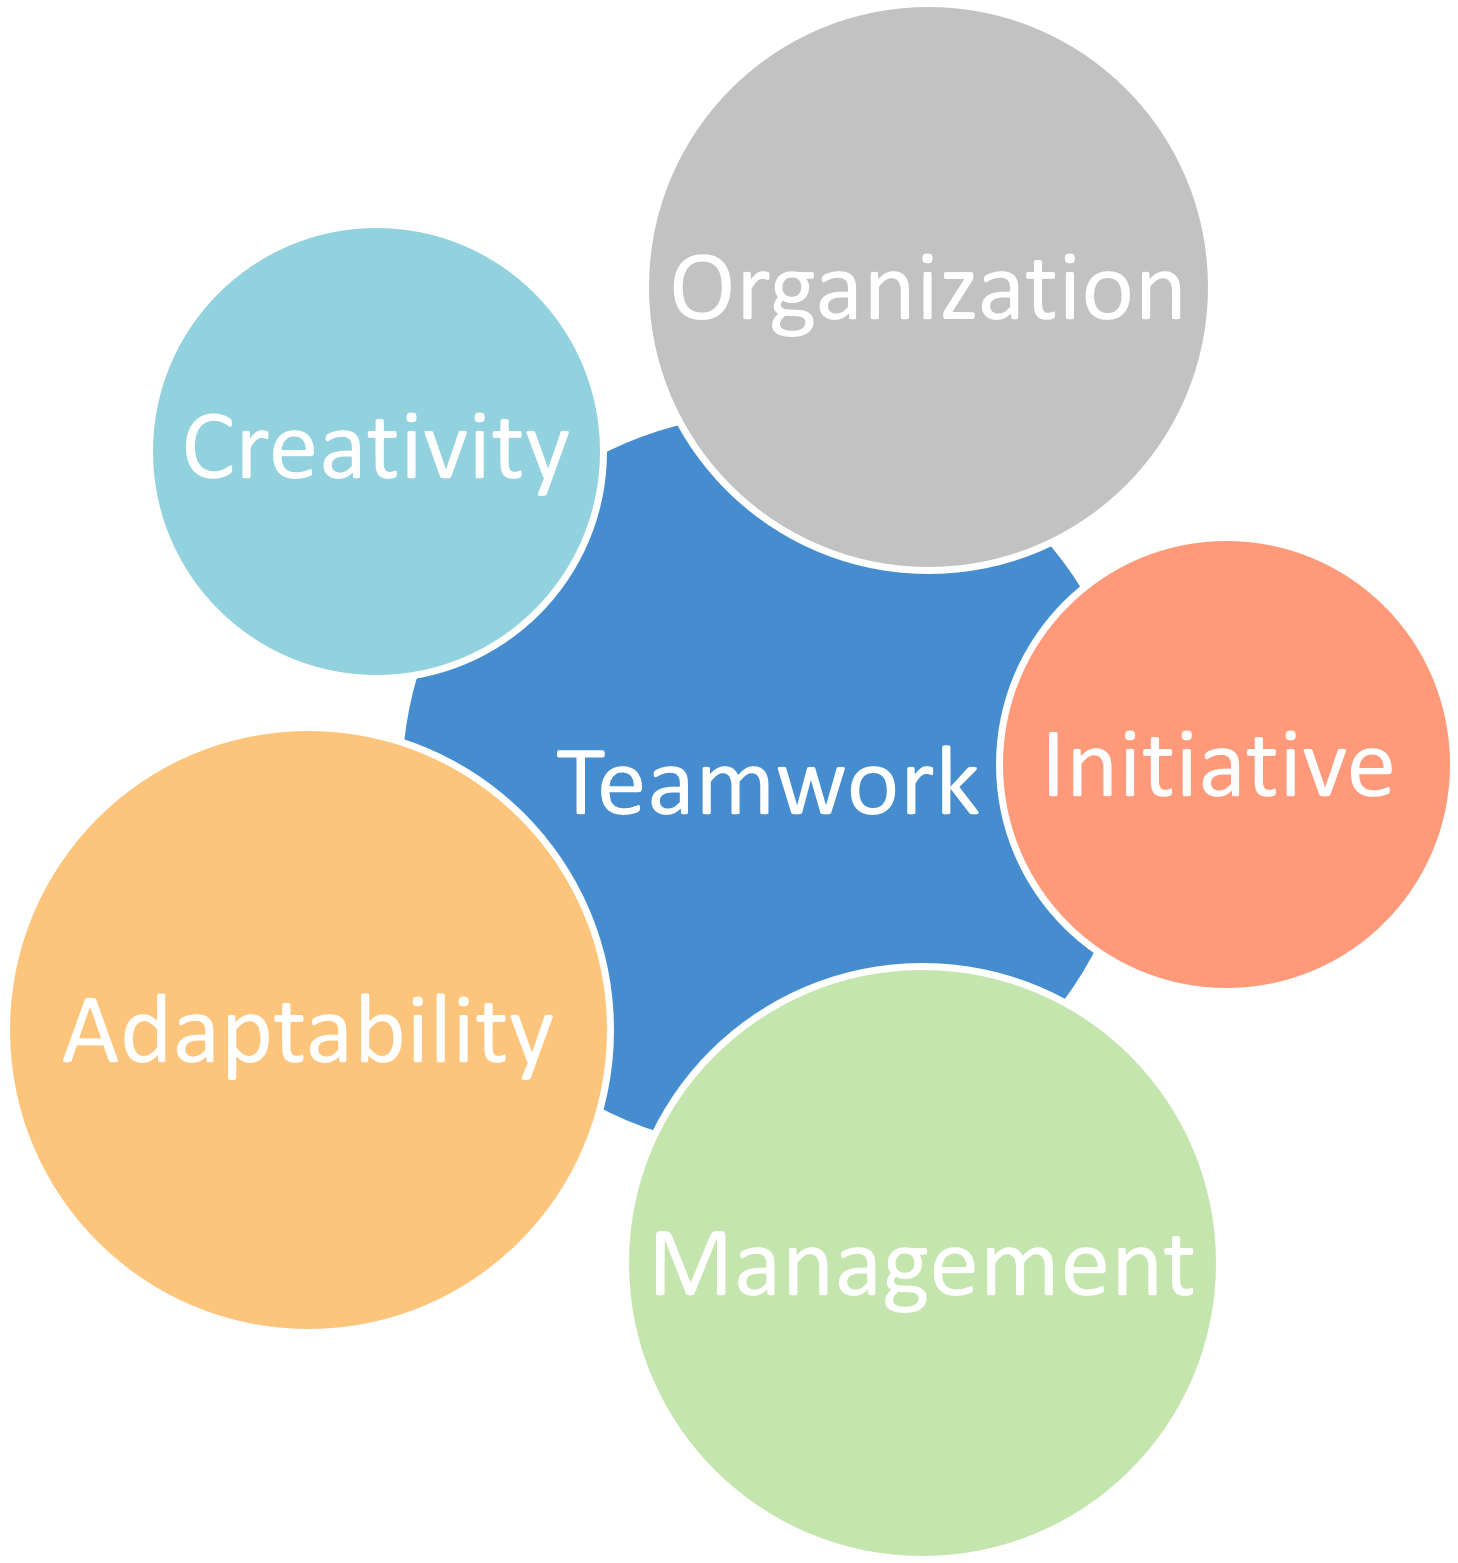
\includegraphics[scale=0.40]{res/img/profileMap_EN.png}\vspace{2.5mm}
\section{CAD / CAM}

\includegraphics[scale=0.40]{res/img/5stars.png}\hspace{1.5mm}\textbf{Catia V5\&V6}

\includegraphics[scale=0.40]{res/img/4stars.png}\hspace{1.5mm}\textbf{Creo 4.0}

\includegraphics[scale=0.40]{res/img/3stars.png}\hspace{1.5mm}\textbf{3D Printing}\section{PLM / PDM}

\includegraphics[scale=0.40]{res/img/4stars.png}\hspace{1.5mm}\textbf{NewPDM}

\includegraphics[scale=0.40]{res/img/3stars.png}\hspace{1.5mm}\textbf{Windchill}\section{FEM / CAE}

\includegraphics[scale=0.40]{res/img/3stars.png}\hspace{1.5mm}\textbf{Ansys Wbench}

\includegraphics[scale=0.40]{res/img/3stars.png}\hspace{1.5mm}\textbf{Abaqus}

\includegraphics[scale=0.40]{res/img/2-5stars.png}\hspace{1.5mm}\textbf{Hyperworks}

\includegraphics[scale=0.40]{res/img/2-5stars.png}\hspace{1.5mm}\textbf{Hypermesh}
\vspace{2.5mm}%\begin{flushleft}
	\emph{Le 23/7/2024} \hspace*{8mm}
	%\end{flushleft}
\end{aside}
\section{IT-Skills}
        \vspace*{-0.45cm}
        \setlength{\columnsep}{-0.3cm}
        \begin{flushleft}
        \begin{multicols}{3}
		\begin{itemize}
		
		\setlength{\itemsep}{5pt}
  		\setlength{\parskip}{0pt}
  		\setlength{\parsep}{0pt}
          
        
\item \large Mobile Development \
\normalsize
\begin{flushleft}


\includegraphics[scale=0.40]{res/img/4stars.png}\hspace{1.5mm}\textbf{Kotlin}\\Room, Firebase, Gson, Jetpack Compose, Retrofit, MVVM, Coroutine\\\vspace{2mm}

\includegraphics[scale=0.40]{res/img/4stars.png}\hspace{1.5mm}\textbf{Flutter}

\includegraphics[scale=0.40]{res/img/4stars.png}\hspace{1.5mm}\textbf{Android}
\end{flushleft}            

\item \large Web Development \
\normalsize
\begin{flushleft}


\includegraphics[scale=0.40]{res/img/4stars.png}\hspace{1.5mm}\textbf{HTML,CSS}

\includegraphics[scale=0.40]{res/img/4stars.png}\hspace{1.5mm}\textbf{JavaScript}
\end{flushleft}            

\item \large Web Frameworks \
\normalsize
\begin{flushleft}


\includegraphics[scale=0.40]{res/img/4stars.png}\hspace{1.5mm}\textbf{Django}

\includegraphics[scale=0.40]{res/img/4stars.png}\hspace{1.5mm}\textbf{Vue.Js}

\includegraphics[scale=0.40]{res/img/3stars.png}\hspace{1.5mm}\textbf{PHP-Laravel}
\end{flushleft}            

\columnbreak
\item \large Back-end / Server \
\normalsize
\begin{flushleft}


\includegraphics[scale=0.40]{res/img/5stars.png}\hspace{1.5mm}\textbf{Python}\\Flask, SQLAlchemy, PyMongo, PyTest, FastAPI, Numpy\\\vspace{2mm}

\includegraphics[scale=0.40]{res/img/3stars.png}\hspace{1.5mm}\textbf{Node.js}

\includegraphics[scale=0.40]{res/img/3stars.png}\hspace{1.5mm}\textbf{Java}

\includegraphics[scale=0.40]{res/img/3stars.png}\hspace{1.5mm}\textbf{\small Nginx,Apache}

\includegraphics[scale=0.40]{res/img/4stars.png}\hspace{1.5mm}\textbf{API}
\end{flushleft}            

\item \large Authentication \
\normalsize
\begin{flushleft}


\includegraphics[scale=0.40]{res/img/4stars.png}\hspace{1.5mm}\textbf{JWT Auth}

\includegraphics[scale=0.40]{res/img/4stars.png}\hspace{1.5mm}\textbf{Firebase}
\end{flushleft}            

\item \large Devops, CI/CD \
\normalsize
\begin{flushleft}


\includegraphics[scale=0.40]{res/img/4stars.png}\hspace{1.5mm}\textbf{Git / GitLab}

\includegraphics[scale=0.40]{res/img/3stars.png}\hspace{1.5mm}\textbf{Docker}

\includegraphics[scale=0.40]{res/img/3stars.png}\hspace{1.5mm}\textbf{Jenkins}

\includegraphics[scale=0.40]{res/img/3stars.png}\hspace{1.5mm}\textbf{Selenium}

\includegraphics[scale=0.40]{res/img/3stars.png}\hspace{1.5mm}\textbf{Cron}
\end{flushleft}            

\columnbreak
\item \large Databases \
\normalsize
\begin{flushleft}


\includegraphics[scale=0.40]{res/img/4stars.png}\hspace{1.5mm}\textbf{MySQL}

\includegraphics[scale=0.40]{res/img/3stars.png}\hspace{1.5mm}\textbf{PostgreSQL}

\includegraphics[scale=0.40]{res/img/4stars.png}\hspace{1.5mm}\textbf{MongoDB}

\includegraphics[scale=0.40]{res/img/3stars.png}\hspace{1.5mm}\textbf{SQLite}
\end{flushleft}            

\item \large Data \
\normalsize
\begin{flushleft}


\includegraphics[scale=0.40]{res/img/4stars.png}\hspace{1.5mm}\textbf{Shiny}

\includegraphics[scale=0.40]{res/img/4stars.png}\hspace{1.5mm}\textbf{Pandas}

\includegraphics[scale=0.40]{res/img/4stars.png}\hspace{1.5mm}\textbf{Matplotlib}

\includegraphics[scale=0.40]{res/img/4stars.png}\hspace{1.5mm}\textbf{Jupyter}
\end{flushleft}            

\item \large AI \& Tools \
\normalsize
\begin{flushleft}


\includegraphics[scale=0.40]{res/img/3stars.png}\hspace{1.5mm}\textbf{Tensorflow}

\includegraphics[scale=0.40]{res/img/3stars.png}\hspace{1.5mm}\textbf{Keras}
\end{flushleft}            

\item \large Others \
\normalsize
\begin{flushleft}


\includegraphics[scale=0.40]{res/img/3stars.png}\hspace{1.5mm}\textbf{Bash}

\includegraphics[scale=0.40]{res/img/4stars.png}\hspace{1.5mm}\textbf{OpenAPI}

\includegraphics[scale=0.40]{res/img/4stars.png}\hspace{1.5mm}\textbf{Jira}
\end{flushleft}            


        \end{itemize}
        \end{multicols}
        %\end{itemize}
        \end{flushleft} \normalsize
        \vspace*{-0.65cm}
\section{Work Experience}
\vspace*{-0.25cm}

\begin{entrylist}
  \entry
    {09/22 - 11/23}
    {Web \& mobile developer}
    {Synapsun, \textit{Lyon, FR}}
    {Full stack web \& Android mobile developments: \hspace*{8mm}Flutter, Python, Kotlin}
\end{entrylist}

\begin{entrylist}
  \entry
    {11/19 - 04/22}
    {R\&D Engineer}
    {Böllhoff (via Davricourt), \textit{Chambéry, FR}}
    {Automotive Mechatronic Product design \& development}
\end{entrylist}

\begin{entrylist}
  \entry
    {11/16 - 09/19}
    {Automotive Design Engineer}
    {Renault (via Bertrandt), \textit{Vélizy, FR}}
    {Underbody \& Engine Compartment Design \& Architecture}
\end{entrylist}

\vspace*{-0.5cm}
\vspace*{0.45cm}
\section{Education - Certifications}
\vspace*{-0.25cm}
\vspace{0.5mm}
\begin{entrylist}
  \entry
    {09/22 - 08/23}
    {Bachelor Degree in Software Design \& Development}
    {EPSI, \textit{Lyon, FR}}
    {RNCP Lvl.6 - Data/IA minor; \hspace{7mm} 09/23: Government Skill Certification}
\end{entrylist}
\vspace*{-0.65cm}
\begin{itemize}
\setlength{\itemsep}{1pt}
\setlength{\parskip}{0pt}
\setlength{\parsep}{0pt}
\begin{multicols}{2}
\item Development: \newline Java, Python, Dart/Flutter, etc.
\columnbreak
\item Data, Databases, etc.
\item Tests \& CI/CD
\end{multicols}
\end{itemize}\vspace{0.5mm}
\begin{entrylist}
  \entry
    {06/22 - 08/22}
    {Web Developer Formation}
    {Epitech, \textit{Paris, FR}}
    {RNCP Lvl.5}
\end{entrylist}

\vspace*{-0.35cm}
\begin{itemize}
\setlength{\itemsep}{1pt}
\setlength{\parskip}{0pt}
\setlength{\parsep}{0pt}

\item PHP, HTML, CSS, JavaScript, Vue.Js, Laravel, Bash, Git
\end{itemize}\vspace{0.5mm}
\begin{entrylist}
  \entry
    {09/13 - 08/16}
    {Master degree in Mechanical Systems Engineering}
    {UTT, \textit{Troyes, FR}}
    {RNCP Lvl.7; Environmental Design \& Industrialization minor}
\end{entrylist}
\vspace{0.5mm}
\begin{entrylist}
  \entry
    {09/11 - 06/13}
    {2-Year Degree in Mechanical Engineering}
    {IUT, \textit{Troyes, FR}}
    {RNCP Lvl.5}
\end{entrylist}
\vspace*{-0.4cm}
\begin{itemize}
\setlength{\itemsep}{1pt}
\setlength{\parskip}{0pt}
\setlength{\parsep}{0pt}
\item Design, Functional dimensioning, enslavement and programming of a robot to take part in the Franch robotic cup.
\end{itemize}
\end{document}